\chapter{Programmbeschreibung}\label{ch:programmbeschreibung}

\section{Programmablaufplan}\label{sec:pap}
Der Ablauf des Programms ist sequenziell und kann daher gut mit Programmablaufplänen dargestellt werden.
Die folgenden Abbildungen beschreiben Teile des Programms.
Abbildung~\ref{fig:diagramm1} zeigt, wie aus wiederholten Benutzereingaben Sätze konstruiert werden.
Die Auswahl eines externen Wörterbuchs wird in Abbildung ~\ref{fig:diagramm2} beschrieben.
In Abbildung~\ref{fig:diagramm3} wird der Ablauf des Explizimodus visualisiert.
Die Ermittlung eines Wortes, aus einem eingegebenen T9-Code, kann in Abbildung~\ref{fig:diagramm4} beobachtet werden.


% \begin{figure}[!h]
%     \centering
%     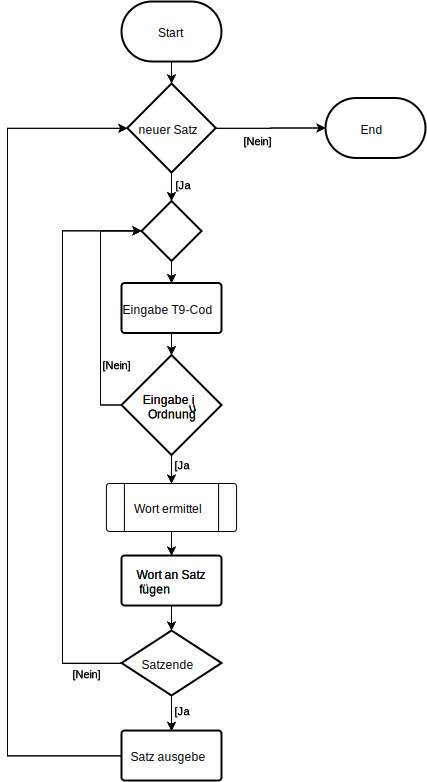
\includegraphics[scale=0.9,width=\textwidth,height=\textheight,keepaspectratio]{Benutzerdialog}
%     \caption{
%         Benutzerdialog: Konstruieren von Sätzen aus Sicht des Anwenders.
% %        Zunächst werden Wörter eingelesen, falls der Satz beendet wird, wird er ausgegeben.
% %        Das Programm wird beendet, falls der finale Satz leer ist und ein Punkt eingegeben wird.
%     }
%     \label{fig:diagramm1}
% \end{figure}

% \begin{figure}[!h]
%     \centering
%     \includegraphics[width=\textwidth,height=\textheight,keepaspectratio]{Einlesen_WBuch1}
%     \caption{
%         Einlesen eines externen Wörterbuchs.
% %        Der Benutzer wird gefragt, ob ein externes Wörterbuch eingelesen werden soll.
% %        Der Benutzer möchte ein externes Wörterbuch einlesen, dann wird jeder Datensatz gelesen, geprüft und in das interne Wörterbuch gespeichert, wenn die Prüfung des Datensatzes erfolgreich war.
% %        Das Einlesen wird abgebrochen, sobald ein Fehler in der Prüfung ist.
% %        Falls die einzulesende Datei nicht gefunden wird, fängt die Methode von vorne an.
% %        Wenn der Benutzer kein externes Wörterbuch nutzen möchte, wird ein neues erstellt.
%     }
%     \label{fig:diagramm2}
% \end{figure}

% \begin{figure}[!h]
%     \centering
%     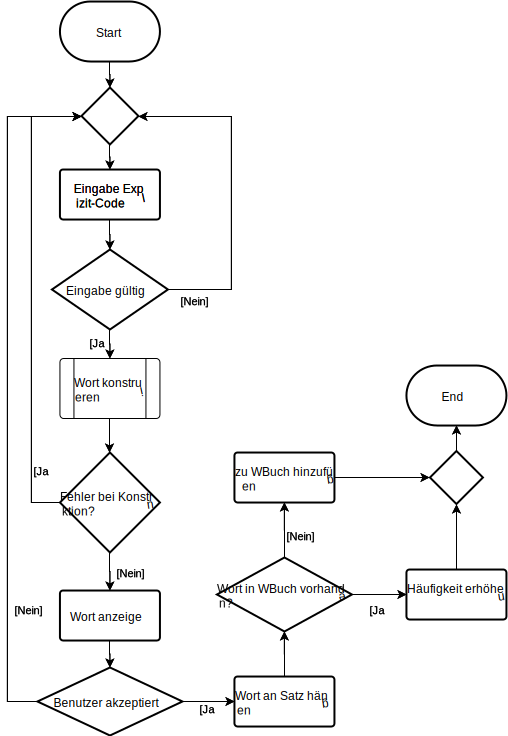
\includegraphics[width=\textwidth,height=\textheight,keepaspectratio]{Explizitmodus}
%     \caption{
%         Ablauf des Explizitmodus.
% %        Zunächst gibt der Benutzer ein Wort in expliziter Darstellung ein.
% %        Dieses wird geprüft und danach konstruiert.
% %        Der Benutzer prüft das konstruierte Wort, falls das Wort dem Wunsch des Benutzers entspricht, wird noch geschaut, ob es im Wörterbuch bereits vorhanden ist.
% %        Wenn es schon vorhanden war, wird die Häufigkeit erhöht, sonst wird das neue Wort mit dem zugehörigen Code und der Häufigkeit eins dem Wörterbuch hinzugefügt.
%     }
%     \label{fig:diagramm3}
% \end{figure}

% \begin{figure}[!h]
%     % \centering
%     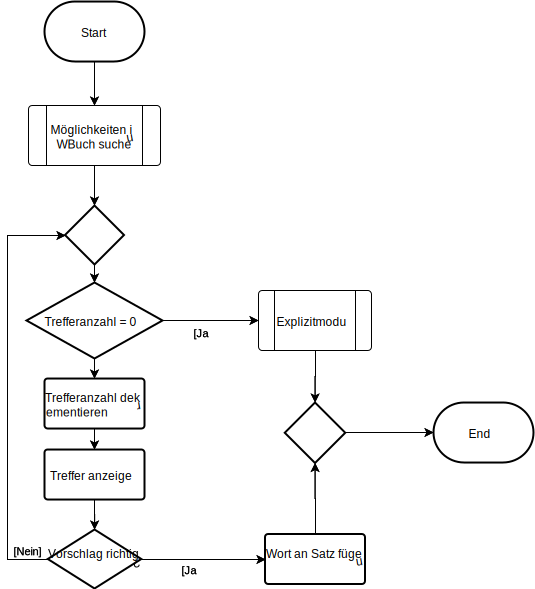
\includegraphics[width=\textwidth,height=\textheight,keepaspectratio]{Wort_ermitteln}
%     \caption{
%         Ermitteln eines Wortes.
% %        Wort ermitteln: Zu Beginn wird im Wörterbuch geschaut, ob der eingegebene Code vorhanden ist.
% %        Die Treffer werden dem Benutzer nacheinander angezeigt, je nach der Benutzerrückmeldung wird der nächste Vorschlag angezeigt oder an den Satz angefügt.
% %        Falls die Trefferanzahl gleich null ist, wird der Benutzer in den Explizitmodus weitergeleitet.
%     }
%     \label{fig:diagramm4}
% \end{figure}


\section{Entwicklungsdokumentation}\label{sec:entwicklerdokumentation}


Es wurden grundsätzlich sprechende Namen für Variablen, Abschnitte und Paragrafen gewählt.
Daher bedarf es nur geringer Dokumentation.
Die Funktionen der einzelnen Paragrafen sind in Tabelle~\ref{tab:prog-strukt} beschrieben.

Wenn Variablen zu einer bestimmten logischen Einheit gehören, haben sie einen passenden Präfix.

\definecolor{fhfarbe}{HTML}{51B2AC}
\definecolor{fhfarbe2}{HTML}{4FAEAB}
\begin{table}[!htb]
    \centering
    \rowcolors{2}{black!5}{white}
    \begin{tabularx}{\textwidth}{X | X }
       \rowcolor{fhfarbe!25}
       Bezeichnung                             & Beschreibung             \\
%       \hline
       MAIN-PROCEDURE & Hauptablauf, in dem einzelne Aufgaben an andere Paragrafen delegiert werden \\
       \rowcolor{fhfarbe!10}
       Vorlauf SECTION & Abschnitt zur Vorbereitung des Programms  \\
       Auswahl-WBuch & Es wird die Auswahl eines externen Wörterbuchs angeboten  \\
       Einlesen-WBuch & Paragraf zum Einlesen eines, zuvor spezifizierten, Wörterbuchs  \\
       Lese-Satz & Verarbeitungsschritt einer einzelnen Zeile eines externen Wörterbuchs   \\
       Init-Explizit-Tab & Initialisierung des strukturellen Aufbaus der Handytastatur  \\
       \rowcolor{fhfarbe!10}
       Hauptlauf SECTION & Abschnitt zur Hauptaufgabe des Programms  \\
       Benutzer-Dialog & Paragraf zum Steuern des Benutzer-Dialogs \\
       Ermittle-Wort & Ermittelt ein Wort aus einem eingegebenen T9-Code  \\
       Wort-Auswahl &  Paragraf schlägt passende Wörter zum eingegebenen T9-Code vor, und ermöglicht eine Auswahl \\
       Finde-Moeglichkeiten & Es werden alle, zum eingegebenen Code passenden, Wörter im Wörterbuch gefunden und zwischengespeichert   \\
       Sortiere-Nach-Haeuf & Bubble-Sort zum Sortieren der zwischengespeicherten Treffer  \\
       Explizit-Eingabe & Steuerung der Eingabe im Explizitmodus  \\
       Suche-Wort-In-WBuch & Prüft, ob ein Wort bereits im Wörterbuch vorhanden ist  \\
       Konstruiere-Wort & Konstruiert ein Wort aus einem eingegebenen Explizit-Code  \\
       Pruefe-Explizit-Eingabe &  Validiert eine Benutzereingabe im Explizitmodus \\
       Pruefe-Eingabe & Validiert eine Benutzereingabe im normalen Modus \\
       \rowcolor{fhfarbe!10}
       Nachlauf SECTION & Abschnitt zum Speichern des Wörterbuchs \\
       Schreibe-WBuch-Sortiert &  Sortiert das Wörterbuch alphabetisch und speichert es in einer Datei \\
    \end{tabularx}
    \caption{Aufgaben der einzelnen logischen Einheiten.}\label{tab:prog-strukt}
\end{table}
